% Final paper: Track B. 11pt, one column, 1-inch margins.
\documentclass[11pt]{article}
\usepackage[utf8]{inputenc}
\usepackage[T1]{fontenc}
\usepackage[spanish,es-nodecimaldot,es-noshorthands]{babel}
\usepackage[margin=1in]{geometry}
\usepackage{amsmath,amssymb,amsthm,booktabs,array,longtable,graphicx}
\usepackage[round]{natbib}
\usepackage[colorlinks=true,allcolors=blue!50!black]{hyperref}
\usepackage{xcolor}
\newtheorem{proposition}{Proposición}
\theoremstyle{definition}\newtheorem{assumption}{Supuesto}
\newcommand{\R}{\mathbb R}
\newcommand{\E}{\mathbb E}
\newcommand{\threshold}{0.640}
\newcommand{\betaZero}{0.130}
\newcommand{\betaOne}{-0.085}
\newcommand{\riskMin}{8.89}
\newcommand{\riskMax}{23.80}
\newcommand{\effortMin}{0.224}
\newcommand{\effortMax}{0.400}
\newcommand{\cohortSlope}{0.130}
\newcommand{\stockSlope}{-0.034}

\title{El precio relativo del crédito como señal de morosidad:\\
\large evaluación óptima, restricciones y composición de la cartera}
\author{Fabián Matías Galarza Chumbe\thanks{Universidad del Pacífico.
Track B, AI and Economic Modeling, 2026-II.
\url{https://github.com/fgalarzac/ai-project}. El plan de investigación con
William Brandon Grados Taco motiva la pregunta. Este modelo y su implementación
son una adaptación para el curso con asistencia de IA declarada en el apéndice.}}
\date{10 de noviembre de 2026. Manuscrito para discusión}
\begin{document}
\maketitle
\begin{abstract}
¿Cuándo informa el precio de créditos nuevos sobre la morosidad futura de un
banco peruano? Resuelvo una decisión de evaluación condicionada en el precio.
Con selección adversa lineal y costo cuadrático, el riesgo marginal es
$a-g^2/c$ solo en el interior. La capacidad limitada lo vuelve $a$ y el piso
de probabilidad lo vuelve cero. Un umbral por opacidad requiere condiciones
adicionales de cruce y monotonía. Al agregar cohortes, la pendiente del ratio
de cartera incorpora un término de composición que puede invertir el signo
del riesgo de originación. Pruebas completas y comprobaciones independientes
delimitan estos resultados. Las simulaciones son ilustrativas; no estimo una
mejora predictiva peruana. La formalización completa mediante el flujo oficial
de Lean y las derivaciones manuscritas personales permanecen pendientes.
\end{abstract}

\section{Problema económico y contribución}
Un supervisor observa el precio al que un banco coloca préstamos nuevos antes
de conocer cómo se comportarán. Cuando una parte de esos préstamos acumula
atrasos, la exposición ya está en el balance. Una brecha de tasas frente a
otros bancos podría aportar información para decidir dónde investigar primero.
La pregunta de la tesis que motiva este trabajo es si esa brecha mejora el
pronóstico de morosidad de la banca múltiple peruana. Aquí desarrollo el
modelo económico que debe preceder a esa evaluación, dentro de Track B.

El signo de la señal no es obvio. Una tasa mayor puede atraer un conjunto de
solicitantes más riesgoso. También aumenta el valor de que un préstamo se
mantenga al día y puede incentivar una evaluación más cuidadosa. Además, el
precio puede reducir el volumen de nuevas colocaciones: si estas son más
riesgosas que la cartera antigua, reducir su peso baja el ratio total aunque
empeore la calidad de cada préstamo nuevo. Es indispensable distinguir estas
tres fuerzas antes de interpretar una regresión predictiva.

La respuesta del modelo tiene condiciones precisas. En una solución interior,
la selección supera a la evaluación si $a>g^2/c$, donde $a$ mide la sensibilidad
de la calidad de solicitantes al precio, $g$ la productividad de evaluar y $c$
su costo marginal creciente. La pendiente de riesgo cambia de signo con la
opacidad únicamente si la diferencia entre esas fuerzas cruza cero. Una
restricción de capacidad puede impedir que opere la respuesta negativa.
Finalmente, trasladar el signo a una cartera requiere controlar cuánto pesan
las cohortes y qué ocurre con los créditos antiguos.

El aporte respecto del avance del tema es doble: una solución global con
restricciones económicamente válidas, y una condición explícita para el
vínculo entre flujos y stocks. Reemplazo el enlace postulado
$NPL=\alpha+\rho q+u$ por una identidad de composición. No se obtiene una
nueva estimación del Perú ni se resuelve competencia estratégica en precios.
Esta delimitación evita llamar evidencia predictiva a una derivada condicional.

\section{Evidencia verificable y medición}
\subsection{Qué se observa y qué no se recibió}
La SBS publica tasas efectivas anuales por empresa y operación. Su metodología,
sección 3, indica promedios de operaciones de los últimos treinta días útiles
ponderados por los montos desembolsados \citep{sbsmetodo}. Son tasas sobre
\emph{flujos}, diferentes de las tasas sobre saldos. Treinta días útiles
pueden superponerse entre cierres mensuales: no equivalen a una cohorte exacta
del mes calendario. Las celdas mejoran comparabilidad, pero no igualan
garantías, plazo exacto, calidad del deudor o relaciones comerciales.

La descomposición de costos de \citet{choy2015}, para 2010--2014, documenta que
costos operativos y riesgo ayudan a explicar las diferencias entre segmentos
peruanos. Por eso una tasa elevada no identifica por sí sola selección
adversa ni una prima de riesgo pura. Una segunda regularidad institucional es
la coexistencia de medidas distintas de calidad: cartera atrasada, atraso
mayor de noventa días y cartera de alto riesgo (CAR). El evento del modelo
debe corresponder a la medida elegida, no a una etiqueta genérica de impago.

El BCRP presenta tanto indicadores de saldo como seguimiento por cosechas en
su Reporte de Estabilidad Financiera de noviembre de 2024, cuadro 2.2 y gráfico
2.7 \citep{bcrp2024}. La Figura~\ref{fig:context} reproduce una transcripción
acotada del cuadro: revela heterogeneidad entre segmentos y justifica cuidar
composición y definición. Su universo es el sistema financiero, más amplio
que banca múltiple. La CAR ajustada incluye castigos de doce meses y no es la
variable dependiente que se propone para la tesis. Esta evidencia motiva el
modelo; no valida sus parámetros ni sus mecanismos.

\begin{figure}[htbp]
\centering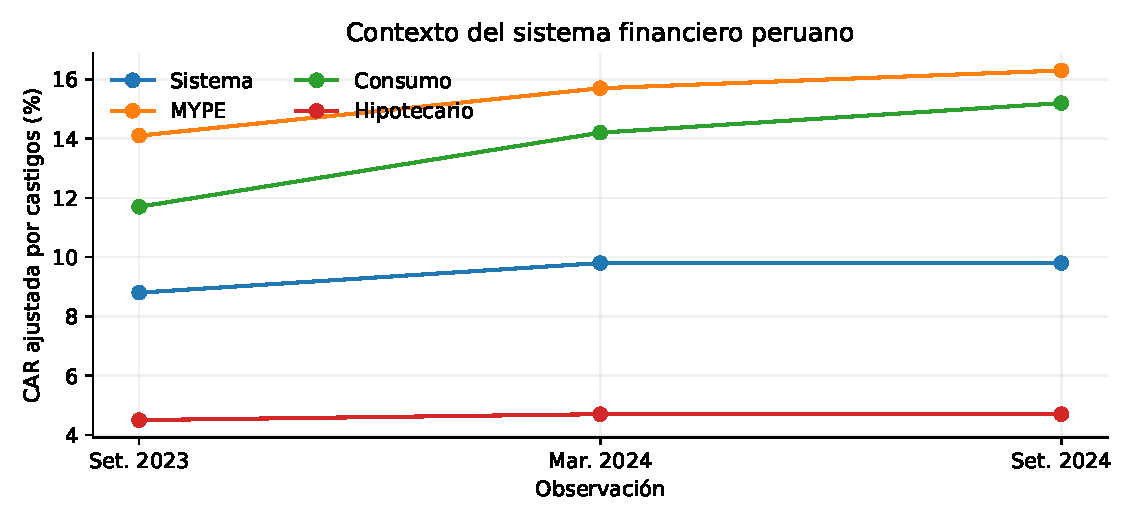
\includegraphics[width=.88\linewidth]{../code/figures/public_context.pdf}
\caption{Contexto observado. CAR ajustada por castigos, porcentaje, sistema
financiero. Fuente: BCRP, Reporte de Estabilidad Financiera, noviembre de 2024,
cuadro 2.2, p. 21. Transcripción en \texttt{code/data/}. No es una estimación
original ni un ratio exclusivo de banca múltiple.}\label{fig:context}
\end{figure}

El plan de Grados y Galarza tiene 24 páginas e incluye cifras para 18 bancos,
porcentajes de varianza, correlaciones y coberturas hasta 2026. No se recibió
la base consolidada ni los scripts que el propio plan dice entregar aparte.
Por tanto, estas cifras permanecen \emph{no verificadas} en esta entrega y
no se reutilizan como hechos confirmados. Tampoco se adopta su afirmación de
que restar pares elimina toda la exposición común al ciclo. La distinción
entre una fuente observada, un cálculo reproducido y una hipótesis importa
para la calidad de la inferencia.

\subsection{Definición principal del precio relativo}
Sea $j$ un banco, $s$ una celda de tipo de crédito, modalidad o tramo de plazo
y moneda, y $t$ la fecha del reporte. Denote por $i_{jst}$ su tasa anual en
decimales y por $b_{st}$ una base común en la misma moneda. Sea
$\mathcal P_{-j,st}$ el conjunto de otros bancos con observación válida y
$n_{-j,st}$ su tamaño. Defino
\begin{equation}\label{eq:D}
D_{jst}=(i_{jst}-b_{st})-
\frac{1}{n_{-j,st}}\sum_{k\in\mathcal P_{-j,st}}(i_{kst}-b_{st})
=i_{jst}-\frac{1}{n_{-j,st}}\sum_k i_{kst}.
\end{equation}
El banco evaluado no entra en su referencia. $D=0.02$ significa dos puntos
porcentuales por encima del promedio de pares. Se usa el promedio simple,
coherente con el plan y transparente cuando no se observan desembolsos por
tramo. No es la tasa promedio del sistema ponderada por operaciones.
Se exigirían al menos tres pares para la aplicación empírica.

La propuesta de octubre utilizaba mediana. La mantengo como sensibilidad
porque es menos sensible a tasas extremas, pero cambia el comparador y puede
cambiar incluso el signo de la brecha. Con tasas de pares hipotéticas de
8, 9, 10 y 25\%, una tasa propia de 12\% está un punto por debajo del promedio
y 2.5 puntos por encima de la mediana. El código comprueba ambas diferencias.
Ninguna medida se elige después de observar el error de pronóstico.

La base común se cancela algebraicamente en ambas definiciones. Sin embargo,
si $i_j=b+\lambda_j z+v_j$, donde $z$ es un shock agregado, queda
$(\lambda_j-\bar\lambda_{-j})z+(v_j-\bar v_{-j})$. Subsisten exposiciones
heterogéneas, fondeo, costos, clientela y márgenes. Los cambios en los pares
también mueven $D$ sin que cambie el banco. No interpreto la resta como
identificación causal ni como eliminación de toda heterogeneidad.

\section{Literatura y mecanismos rivales}
\citet{morgan2003} es el antecedente empírico más próximo: encuentra contenido
predictivo de las tasas de nuevos préstamos comerciales e industriales de
Estados Unidos para su desempeño y calificaciones supervisoras. Es un artículo
publicado en 2003, no un preprint. El resumen editorial permite verificar el
alcance; no atribuyo una magnitud o un diseño de identificación que no haya
reproducido. La aplicación peruana con promedios por banco y celda y una
variable de saldo es una pregunta diferente, no una consecuencia del hallazgo.

En teoría, \citet{stiglitz1981}, p. 393, explica que el precio puede modificar
la composición y los incentivos de quienes solicitan crédito. Aquí resumo
el primer canal mediante una pendiente positiva de riesgo previo. No reproduzco
su equilibrio de racionamiento. \citet{broecker1990} estudia pruebas imperfectas
y competencia entre bancos; \citet{ruckes2004} relaciona selección crediticia
y competencia con perspectivas económicas. \citet{dellariccia2006} distingue
regímenes de evaluación y agrupación de prestatarios. Son artículos publicados.
El modelo de este curso utiliza ingredientes conocidos para construir una
descomposición explicable, no reclama prioridad general en economía bancaria.

La literatura peruana de pronóstico también importa. \citet{yamunaque2024}
figura como Documento de Trabajo 2024-015 en el catálogo primario del BCRP,
consultado el 10 de noviembre de 2026. Se cita con ese estado editorial; no se
confirmó una versión de revista en las fuentes primarias consultadas. No es
evidencia de que nuestro indicador funcione. \citet{clark2007} proporciona una
comparación de modelos predictivos anidados, relevante para un trabajo empírico
posterior. No se calcula aquí una prueba ni un valor $p$.

Los mecanismos rivales tienen implicaciones que ayudan a diseñar esa prueba.
Si domina selección, precios altos anteceden peor calidad de nuevas cosechas,
manteniendo constante la evaluación. Si domina evaluación, el precio alto
debe acompañarse de mayor esfuerzo efectivo o mejor documentación y menor
riesgo posterior, salvo que la capacidad esté saturada. Si domina composición,
el cambio de signo aparece al agregar al saldo y depende de la participación
de colocaciones recientes. Los costos de fondeo o venta cruzada pueden generar
brechas sin estos patrones. Con promedios públicos será difícil separarlos;
harían falta, idealmente, datos de cosechas, rotación, evaluación y garantías.

\section{Ambiente y decisión del banco}\label{sec:model}
\subsection{Agentes, información, unidades y cronología}
El único agente que optimiza en este modelo es un banco neutral al riesgo.
Los solicitantes y los bancos pares determinan una calidad y una referencia
reducidas; no se modela su juego estratégico. El supervisor observa $D$ y más
tarde un ratio de cartera, pero no el esfuerzo ni toda la composición de riesgo.
La opacidad $\kappa\in[0,1]$ es una característica exógena del segmento: un
valor mayor representa menor información verificable inicial. No se estima
este índice ni se equipara automáticamente microempresa con opacidad alta.

La cronología es: primero se fijan segmento, tecnología y precio observado;
después se forma el conjunto de solicitantes y el banco observa su riesgo
medio; luego elige esfuerzo antes de originar; finalmente se realiza el
estado crediticio y se observa la cartera al horizonte $h$. El banco conoce
los parámetros al decidir. La incertidumbre de desempeño permanece y se
integra en su objetivo. El precio es un argumento del problema de continuación,
no una variable resuelta en equilibrio.

$q^0$ y $q$ son probabilidades sin unidades, referidas al mismo evento y
horizonte para una cohorte estandarizada. $e$ y $\kappa$ son índices. $D$ se
mide en unidades de tasa anual decimal. Los pagos y costos se normalizan por
sol de crédito. La sensibilidad monetaria del premio de desempeño a una unidad
de $D$ se normaliza a uno. Esto es una simplificación de remuneración, no una
conversión exacta de tasas efectivas a cualquier plazo contractual.

\begin{assumption}[Selección y dominio]\label{as:selection}
Para cada $\kappa$ fijo, $a=a(\kappa)>0$, $\bar q\in(0,1)$ y $D$ pertenece
a un intervalo compacto $\mathcal D$. La probabilidad previa es
$q^0(D,\kappa)=\bar q+a(\kappa)D\in[0,1]$ en todo $\mathcal D$.
\end{assumption}
La forma afín es una aproximación local al cambio de solicitantes. Una subida
de un punto porcentual empeora su probabilidad en $0.01a$, no en $a$ puntos.
No se extrapola fuera del dominio admisible. La pendiente positiva representa
selección adversa, no una ley empírica universal ni una respuesta derivada de
un problema explícito de cada deudor.

\begin{assumption}[Tecnología, capacidad y costo]\label{as:technology}
$g=g(\kappa)>0$, $c=c(\kappa)>0$ y $\bar e\ge0$ son finitos. Para un volumen
normalizado de créditos, $q(D,e,\kappa)=q^0(D,\kappa)-g(\kappa)e$ y el costo
es $c(\kappa)e^2/2$. La elección factible cumple
\[
0\le e\le u(D,\kappa):=\min\{\bar e,q^0(D,\kappa)/g(\kappa)\}.
\]
\end{assumption}
El límite $q^0/g$ evita probabilidades negativas. La capacidad $\bar e$ puede
representar personal o tiempo de verificación. Evaluar incluye comprobación
y condiciones contractuales que reducen el riesgo de los créditos colocados.
El modelo mantiene el volumen fijo respecto del esfuerzo: no estudia la
composición endógena de rechazos ni su costo de reemplazo. Si evaluar elimina
solicitantes sin reemplazo, el volumen dependería de $e$ y la solución cambiaría.
La tecnología lineal puede llegar a riesgo cero, una frontera matemática cuyo
realismo es limitado; no se presenta como objetivo factible de un supervisor.

\begin{assumption}[Remuneración y problema condicionado]\label{as:payoff}
El premio normalizado por desempeño es $R(D)=\bar R+D>0$ y $F$ es un costo
por unidad independiente de $e$. El banco resuelve
\begin{equation}\label{eq:problem}
\max_{e\in[0,u(D,\kappa)]}\pi(e;D,\kappa)
=[1-q^0(D,\kappa)+g(\kappa)e]R(D)-F-\frac{c(\kappa)}2e^2.
\end{equation}
El precio, la referencia de pares y $\kappa$ se mantienen fijos al evaluar
desviaciones de esfuerzo.
\end{assumption}
El costo $F$ no afecta el óptimo de esfuerzo. Un volumen estrictamente
positivo que multiplique todo el objetivo tampoco lo afecta si no depende
de $e$. La participación o decisión de no prestar no está resuelta: el
resultado se refiere a una unidad que el banco ya contempla originar.
La remuneración supone que evitar el evento adverso mejora el pago esperado.
Recuperaciones, seguros y garantías que varían con precio o esfuerzo exigirían
modificar este premio. El horizonte del evento y el flujo contractual deben
ser compatibles en una implementación empírica.

\section{Resultados y demostraciones completas}
\subsection{Evaluación óptima con todas sus restricciones}
\begin{proposition}[Solución global y pendientes por régimen]\label{p:global}
Bajo los Supuestos~\ref{as:selection}--\ref{as:payoff}, existe un único máximo
en \eqref{eq:problem}. Es
\begin{equation}\label{eq:opt}
e^*=\min\left\{\frac{gR(D)}c,\bar e,\frac{q^0(D)}g\right\},\qquad
q^*=\max\left\{0,q^0(D)-g\min\left\{\bar e,\frac{gR(D)}c\right\}\right\}.
\end{equation}
Para $\kappa$ fijo, en cualquier intervalo abierto con desigualdades estrictas
que mantengan el régimen, las pendientes son
\begin{equation}\label{eq:regimes}
\frac{\partial q^*}{\partial D}=
\begin{cases}
a-g^2/c,&gR/c<\bar e\ \text{y}\ gR/c<q^0/g,\\
a,&\bar e<gR/c\ \text{y}\ \bar e<q^0/g,\\
0,&q^0/g<gR/c\ \text{y}\ q^0/g<\bar e.
\end{cases}
\end{equation}
Si $\bar e=0$, $e^*=0$ y $q^*=q^0$, con pendiente $a$ en el interior del
dominio de $D$. En empates de restricciones la solución es continua y se usan
derivadas laterales; una derivada ordinaria puede no existir.
\end{proposition}
\begin{proof}
El intervalo factible es no vacío, cerrado y acotado porque $q^0\ge0$, $g>0$
y $\bar e\ge0$. El objetivo es continuo, así que alcanza un máximo. Si $u=0$
solo hay una elección. Si $u>0$, $\pi_{ee}=-c<0$ da concavidad estricta y a
lo sumo un máximo. Para encontrarlo sin confundir una FOC con suficiencia,
defina $z=gR/c>0$ y complete el cuadrado:
\[
\pi(e)=(1-q^0)R-F+\frac{(gR)^2}{2c}-\frac c2(e-z)^2.
\]
Maximizar equivale a minimizar la distancia al punto positivo $z$. Si $z<u$,
la distancia cero se alcanza solo en $e=z$. Si $z\ge u$, la distancia cae
estrictamente hasta $e=u$ y ese es el único máximo. Esto también prueba el
caso $z=u$. Por tanto $e^*=\min\{z,u\}$, que produce la primera fórmula.
Restar $ge^*$ de $q^0$ y distinguir si $q^0/g$ es la menor cota produce la
segunda. Ambas probabilidades pertenecen a $[0,1]$: $q^*\ge0$ por la cota y
$q^*\le q^0\le1$ porque $e^*\ge0$.

En el primer régimen, $q^*=\bar q+aD-(g^2/c)(\bar R+D)$, y derivar con
$a,g,c$ fijos da $a-g^2/c$. En el segundo $q^*=\bar q+aD-g\bar e$ y la
pendiente es $a$. En el tercero $q^*=0$ en un entorno y su derivada es cero.
Con capacidad nula la fórmula es inmediata. Mínimos y máximos de funciones
continuas son continuos, lo que prueba continuidad incluso en empates. Las
expresiones adyacentes determinan las pendientes laterales donde hay cambio
de régimen. No se requiere que esas pendientes coincidan.
\end{proof}

La intuición de $g^2/c$ tiene dos pasos: un mayor precio eleva el esfuerzo en
$g/c$ en el interior y cada unidad de esfuerzo reduce riesgo en $g$. Cuando
la capacidad está agotada, la primera respuesta desaparece. En consecuencia,
un banco con alta productividad puede mostrar pendiente positiva si enfrenta
capacidad escasa. La condición $g^2/c>a$ por sí sola no basta globalmente.

\subsection{Qué requiere un umbral por opacidad}
Defina $H(\kappa)=g(\kappa)^2/c(\kappa)$ y
$\beta(\kappa)=a(\kappa)-H(\kappa)$.
\begin{assumption}[Condiciones suficientes para el cruce]\label{as:cross}
En $\kappa\in[0,1]$, $a,g,c$ son continuas y positivas. La función
$a-H$ es estrictamente decreciente y satisface $a(0)>H(0)$ y $a(1)<H(1)$.
Al precio $D_0$ que se compara se cumplen estrictamente las dos condiciones
de interioridad de la primera línea de \eqref{eq:regimes} para todo $\kappa$.
\end{assumption}
\begin{proposition}[Umbral condicional]\label{p:threshold}
Bajo los Supuestos~\ref{as:selection}--\ref{as:cross}, existe un único
$\kappa^*\in(0,1)$ con $\partial_Dq^*(D_0,\kappa^*)=0$. La derivada es
positiva para $\kappa<\kappa^*$ y negativa para $\kappa>\kappa^*$.
\end{proposition}
\begin{proof}
Como $c$ no se anula, $H=g^2/c$ y $\beta=a-H$ son continuas. Los signos
opuestos en los extremos y el teorema del valor intermedio dan un cero en
$(0,1)$. Si hubiera dos ceros, la monotonía estricta exigiría que el segundo
fuera menor que el primero en valor funcional, una contradicción. Para un
punto menor que el cero, la monotonía da $\beta(\kappa)>\beta(\kappa^*)=0$;
para uno mayor da la desigualdad inversa. La interioridad permite aplicar
la primera línea de la Proposición~\ref{p:global} en cada $\kappa$.
\end{proof}

El Supuesto~\ref{as:cross} es una restricción económica contrastable, no el
significado de opacidad. Si las funciones son diferenciables,
\begin{equation}\label{eq:logs}
\frac{H'}H=2\frac{g'}g-\frac{c'}c.
\end{equation}
Por ejemplo, información inicial escasa podría dejar más margen para
verificación adicional, pero no demuestra $g'>0$. Si el acceso a información
es más difícil, es plausible $g'\le0$ y $c'\ge0$, con $H'\le0$. Puede no
haber cruce, o puede haberlo si $a$ cae suficientemente rápido. Ni $H'>0$ es
necesario por sí solo ni la mera continuidad asegura unicidad. Un criterio
suficiente más fuerte, usado en octubre, es $a'<0$, $H'>0$ y cruce de extremos.
El resultado final solo exige que $a-H$ decrezca estrictamente. La sensibilidad
estudia explícitamente una tecnología que empeora con opacidad.

\subsection{El puente entre una cohorte y el saldo de cartera}
Fijemos un horizonte $h$. $B_0>0$ es el saldo de créditos antiguos todavía
vigente en esa fecha y $m_0\in[0,1]$ su proporción en el estado de atraso
elegido. $B(D)>0$ es el saldo de la cohorte nueva que permanece en cartera a
$h$, después de amortización normal. Denote $w(D)=B(D)/(B_0+B(D))$.

\begin{assumption}[Contabilidad y maduración]\label{as:stock}
Al horizonte, el saldo de cada cohorte es determinista o se trata como
exposición de una población continua. El riesgo $q^*(D)$ coincide con la
fracción esperada de su saldo en el evento crediticio elegido, condicional
a seguir en cartera. La amortización y el tamaño del crédito no seleccionan
riesgo adicional no recogido en $q^*$. $B_0,m_0$ son constantes al variar $D$;
$B(D)>0$ es diferenciable. No hay castigos, ventas de cartera ni
reclasificaciones que alteren esta identidad en el ejercicio.
\end{assumption}
El supuesto hace explícito lo que faltaba en el enlace de octubre. Una
probabilidad de impago de por vida no equivale a la probabilidad de figurar
con atraso mayor de noventa días en una fecha dada. Hay que definir horizonte,
maduración, persistencia del atraso y permanencia del saldo. Si esos procesos
cambian con $D$, deben incluirse en $q^*$ o en la contabilidad ampliada.

\begin{proposition}[Transmisión y composición]\label{p:stock}
Bajo los Supuestos~\ref{as:selection}--\ref{as:payoff} y~\ref{as:stock}, el
ratio esperado de cartera es $M(D)=(1-w)m_0+wq^*(D)$. En cualquier régimen
diferenciable, escribiendo $\beta_D=\partial_Dq^*(D)$,
\begin{equation}\label{eq:stock}
M'(D)=w\beta_D+w'(q^*-m_0).
\end{equation}
Si $B$ es constante, el signo es el de $\beta_D$. Si $\beta_D\ne0$ y
$|w'(q^*-m_0)|<w|\beta_D|$, el signo también se conserva.
Con $B(D)=B_1e^{-\varepsilon D}$, $B_1>0$, $\varepsilon\ge0$,
\begin{equation}\label{eq:composition}
M'=w\{\beta_D-\varepsilon(1-w)(q^*-m_0)\}.
\end{equation}
En particular, $\beta_D>0$ y $q^*>m_0$ generan $M'<0$ si y solo si
$\varepsilon(1-w)(q^*-m_0)>\beta_D$.
\end{proposition}
\begin{proof}
El saldo esperado en atraso es $B_0m_0+Bq^*$. Dividirlo por el saldo
determinista $B_0+B$ produce la expresión de $M$; no se sustituye sin
justificación una esperanza de ratios por un ratio de esperanzas. La regla
del producto da $M'=-w'm_0+w'q^*+w\beta_D$, que es \eqref{eq:stock}.
Con $B$ constante, $w'=0$ y $w>0$, así que se conserva el signo, incluido
el caso cero. Si $\beta_D\ne0$, un término de magnitud estrictamente menor
que $w|\beta_D|$ no puede cambiar el signo de $w\beta_D$.

La regla del cociente da $w'=B'B_0/(B_0+B)^2$. Como $B'=-\varepsilon B$,
$w'=-\varepsilon w(1-w)$. Sustituir produce \eqref{eq:composition}.
Dado que $w>0$, $M'<0$ equivale exactamente a que el término entre llaves
sea negativo; al despejar se obtiene la última condición. Todas las
operaciones se realizan en un régimen donde $q^*$ es diferenciable.
\end{proof}

Esta proposición permite ver la dilución de una cohorte pequeña, pero también
un mecanismo distinto: reemplazar créditos antiguos seguros por nuevos más
riesgosos. Si el precio sube y la cohorte nueva pierde peso, el ratio total
puede mejorar mientras empeora su riesgo individual. El signo del coeficiente
predictivo de un ratio de saldo no distingue automáticamente evaluación de
composición. Si $m_0$ cambia con precio, se suma $(1-w)m_0'$; si $B_0$ cambia,
tampoco vale la fórmula particular de $w'$. Son exclusiones sustantivas.

\section{Simulaciones, contraejemplos y sensibilidad}\label{sec:sim}
Todos los parámetros siguientes son ilustrativos, sin ajuste al Perú.
En el escenario interior fijo $\bar q=0.28$, $\bar R=1.10$,
$\bar e=0.50$, $D\in[-0.10,0.10]$ y
\[
a(\kappa)=0.18e^{-0.8\kappa},\quad
g(\kappa)=\sqrt{0.05}e^{0.8\kappa},\quad c(\kappa)=e^{0.4\kappa}.
\]
La amplitud de diez puntos porcentuales facilita ver mecanismos y no pretende
describir variación habitual observada. $F$ se normaliza a cero porque no
afecta esfuerzo. La escala de riesgo, relativamente alta, exhibe un conjunto
factible amplio y no es una calibración de morosidad peruana.

\subsection{Cruce condicionado y su fracaso}
Aquí $H=0.05e^{1.2\kappa}$ y $\beta=0.18e^{-0.8\kappa}-0.05e^{1.2\kappa}$.
Igualar fuerzas, dividir por $0.05e^{-0.8\kappa}>0$ y tomar logaritmos da
$\kappa^*=\log(3.6)/2=\threshold$. Las pendientes de extremos son
\betaZero{} y \betaOne{}. En una malla de 1001 opacidades por 121 precios,
el esfuerzo está entre \effortMin{} y \effortMax{}, y el riesgo entre
\riskMin\% y \riskMax\%. El código verifica además la factibilidad de
cada punto. Estas cifras proceden de \texttt{code/output/numbers.tex}.

\begin{figure}[htbp]
\centering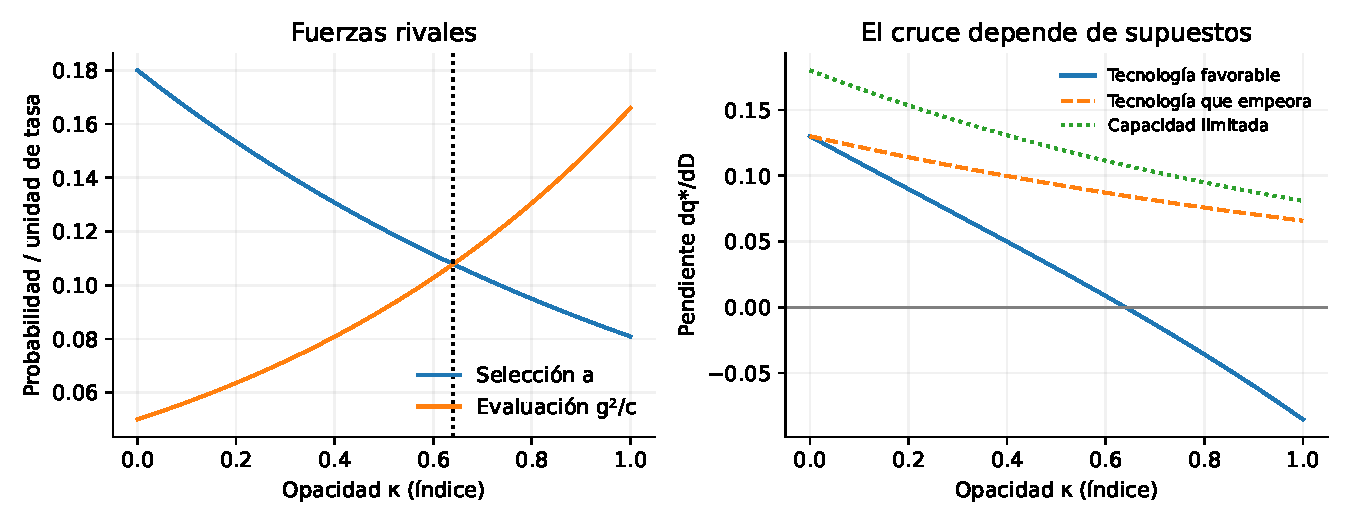
\includegraphics[width=\linewidth]{../code/figures/mechanisms.pdf}
\caption{Selección, evaluación y supuestos del cruce. La tecnología alternativa
usa $g=\sqrt{0.05}e^{-0.4\kappa}$; el costo sigue aumentando. Capacidad limitada:
$\bar e=0.08$. Fuente: simulación ilustrativa, \texttt{code/verify.py}.
Una unidad de pendiente se mide por unidad de tasa decimal.}\label{fig:mechanisms}
\end{figure}

La Figura~\ref{fig:mechanisms} incluye un escenario igualmente admisible en
el que $g$ cae: $H=0.05e^{-1.2\kappa}$. Entonces
$a/H=3.6e^{0.4\kappa}>1$ en todo el intervalo y no hay reversión. El código
también muestra que una capacidad de 0.08 mantiene pendiente positiva aunque
la tecnología de evaluación sea favorable. Son contraejemplos a una lectura
incondicional de que la opacidad invierte el signo.

\subsection{Esquinas y estabilidad}
La Figura~\ref{fig:corners} utiliza dos configuraciones adicionales.
Con $\bar q=0.35$, $a=0.04$, $g=0.4$, $c=1$ y $\bar e=0.44$, la restricción
de capacidad empieza a operar en $D=0$. A la izquierda, la pendiente de riesgo
es $0.04-0.16=-0.12$; a la derecha es $0.04$. La solución es continua, pero
no diferenciable en ese punto. En el segundo caso $\bar q=0.04$, $a=0.04$,
$g=0.5$, $c=1$ y $\bar e=1$ llevan al piso de riesgo, que detiene reducciones
adicionales. La igualdad de una FOC sin restricciones daría probabilidades
negativas en ese ejemplo y sería una solución inválida.

\begin{figure}[htbp]
\centering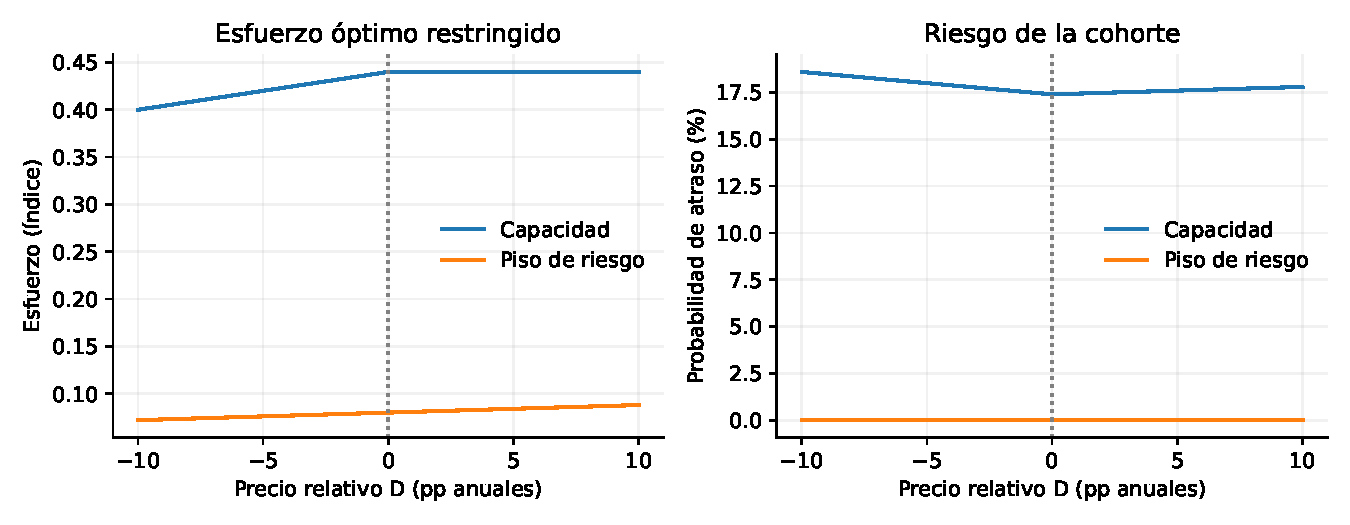
\includegraphics[width=.95\linewidth]{../code/figures/corners.pdf}
\caption{Esfuerzo y riesgo con capacidad y piso de probabilidad. $D$ en puntos
porcentuales anuales, riesgo en porcentaje. Fuente: \texttt{code/verify.py},
parámetros hipotéticos. El piso cero describe una frontera de la tecnología
lineal y no una recomendación de política.}\label{fig:corners}
\end{figure}

La solución analítica se compara con un optimizador acotado de SciPy que evalúa
directamente el objetivo e incluye ambos extremos como candidatos. De 1500
sorteos con semilla 20261110, 1495 son admisibles: 765 interiores, 293 de
capacidad y 437 de piso de riesgo. La máxima diferencia de esfuerzo fue
menor que $4\times10^{-8}$, con tolerancia exigida de $2\times10^{-6}$.
Las pendientes se contrastan con diferencias centrales de paso $10^{-6}$
solo cuando los tres puntos conservan régimen; el error máximo fue menor
que $1.1\times10^{-10}$. Se comprueba capacidad nula y se rechazan parámetros
con probabilidades inválidas, costo nulo, productividad negativa o pago no
positivo. No se usan \texttt{assert} que desaparezcan al ejecutar Python con
optimización: una falla necesaria lanza una excepción.

\subsection{Contraejemplo de composición}
En $\kappa=0$, $D=0$, la evaluación interior da $q^*=0.225$ y
$\beta_D=\cohortSlope$. Tome $B_0=4$, $B_1=1$, $m_0=0.10$ y
$\varepsilon=3$. Así $w=0.2$ y
\[
M'=0.2[0.13-3(0.8)(0.225-0.10)]=\stockSlope<0.
\]
Todas las probabilidades y saldos son válidos. Una subida de un punto
porcentual tiene respuesta local de riesgo nuevo de 0.13 puntos porcentuales,
pero respuesta del ratio total de $-0.034$ puntos porcentuales. Son derivadas
locales, no efectos de un cambio discreto grande ni estimaciones causales.

\begin{figure}[htbp]
\centering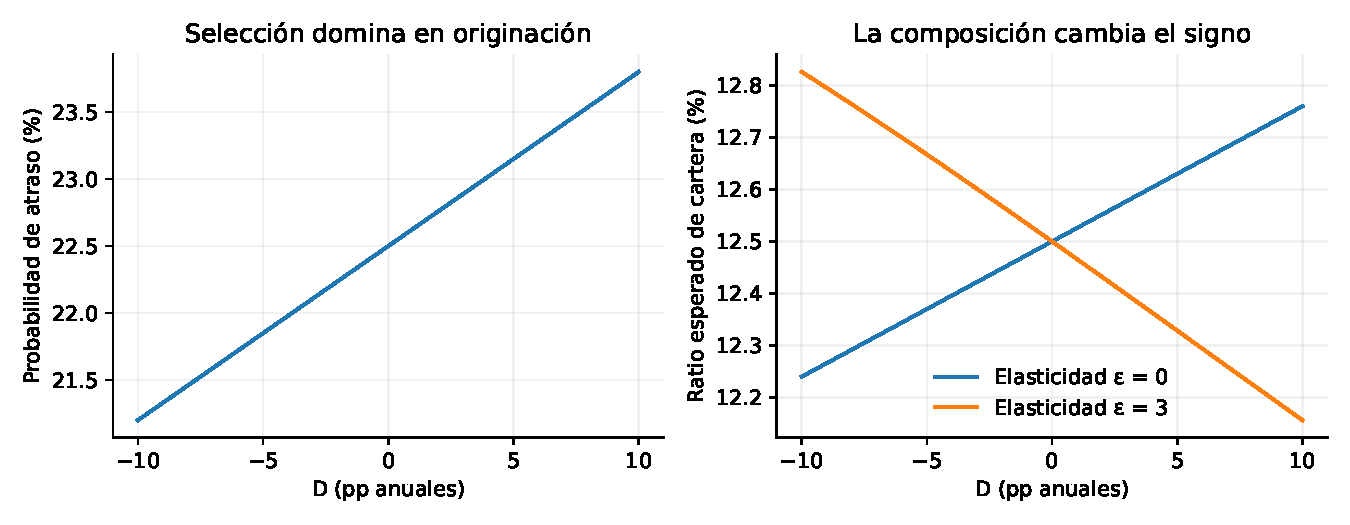
\includegraphics[width=\linewidth]{../code/figures/stock_composition.pdf}
\caption{Un mismo riesgo de cohorte puede asociarse con pendientes de saldo
opuestas. Con peso fijo ($\varepsilon=0$), el signo se transmite. Con volumen
sensible ($\varepsilon=3$), la composición domina. Fuente: simulación
ilustrativa, \texttt{code/verify.py}.}\label{fig:stock}
\end{figure}

La Proposición~\ref{p:stock} se contrasta en 51 valores de opacidad, 25 precios
y cuatro elasticidades, siempre con derivadas bien definidas. El máximo error
frente a diferencias finitas fue inferior a $3\times10^{-11}$. SymPy comprueba
por separado la regla del producto y la derivada del peso exponencial. Esta
doble comprobación reduce el riesgo de repetir un mismo error en una fórmula
y su implementación, aunque no reemplaza una prueba formal.

\begin{figure}[htbp]
\centering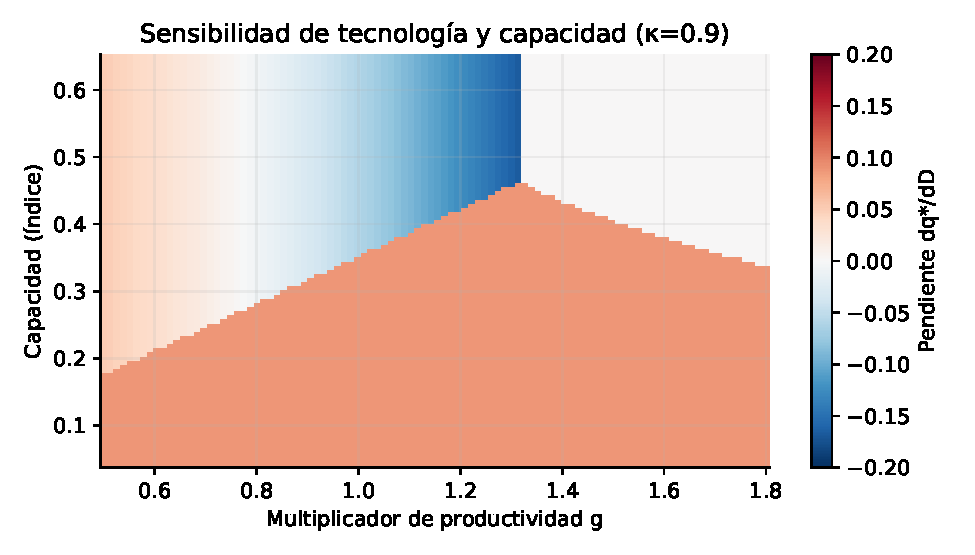
\includegraphics[width=.80\linewidth]{../code/figures/sensitivity.pdf}
\caption{Sensibilidad de la pendiente a productividad y capacidad con
$\kappa=0.9$. El mapa incluye los regímenes efectivos, incluido el piso de
riesgo; no extrapola una FOC interior fuera de su dominio. Fuente:
\texttt{code/verify.py}, simulación hipotética.}\label{fig:sensitivity}
\end{figure}

El mapa de la Figura~\ref{fig:sensitivity} varía capacidad y productividad,
manteniendo el resto de parámetros. Mejor productividad no implica una
pendiente negativa ilimitada: la saturación en riesgo cero la vuelve cero.
El ejercicio identifica regiones del modelo, no frecuencias con que ocurren
en bancos peruanos. Sin datos de evaluación no se puede asignar un banco a
una región a partir de su tasa observada.

\section{Interpretación predictiva, límites y agenda empírica}
\subsection{Tres afirmaciones distintas}
La derivada $\partial_Dq^*$ es una estática comparativa condicional: mantiene
primitivas, referencia y régimen al variar precio y permite reoptimizar
esfuerzo. Un coeficiente predictivo de $M_{t+h}$ sobre $D_t$ resume una
distribución conjunta de precios, tecnología, composición y shocks. Un
efecto causal de imponer un precio requiere identificar una intervención y
resolver las respuestas de demanda y de otros bancos. Ni el primero implica
el segundo ni el segundo identifica el tercero.

No se ha resuelto la etapa de precios. La continuidad y un conjunto compacto
pueden asegurar un máximo para un problema externo bien especificado, pero
no caracterizan su unicidad ni un equilibrio oligopólico. En este trabajo no
se añade una demanda estratégica solo para aparentar cierre. La curva
condicional es útil para organizar interpretaciones, pero no determina qué
variación de $D$ se observará ni su endogeneidad. Tampoco se deriva el bienestar
del deudor ni una regla óptima de supervisión.

\subsection{Qué podría comprobar un ejercicio futuro}
El diseño principal sería banco-mes, con precio por celda agregado usando
pesos de saldo rezagados y cobertura explícita. Se conservaría el horizonte
principal de doce meses del plan como elección de diseño, sin atribuirlo a
una equivalencia exacta entre pérdida regulatoria y atraso. La mora mayor de
noventa días sería una variable objetivo separada de la mora contable.
Se compararía un pronóstico con morosidad pasada y ciclo frente a su ampliación
con $D$. La referencia de pares y el spread propio se evaluarían en modelos
que respeten $S=D+C$: incluir los tres genera colinealidad exacta.

Antes de ejecutar haría falta verificar cobertura y fechas de publicación
reales, sin adoptar las del plan como hechos. En un origen $t$, entrenamiento
solo incluiría pares cuyo resultado a $t+h$ ya fue publicado; el extremo de
la ventana debe purgar los horizontes aún desconocidos. Los pesos, escalas,
posición habitual y tratamiento de faltantes se estimarían con pasado
disponible. Las decisiones se fijarían en entrenamiento, incluyendo mínimo
de pares y alternativa mediana. Revisiones históricas de datos convierten una
evaluación en pseudo tiempo real si no hay vintages archivados.

La comparación fuera de muestra usaría los mismos bancos y fechas para ambos
modelos, pérdidas agregadas por origen que respeten dependencia entre bancos,
y corrección por errores superpuestos en horizontes largos. Clark--West sería
una opción para modelos anidados bajo sus condiciones. El criterio de una
reducción de 5\% de la raíz del error del plan es una meta previamente elegida,
no algo demostrado por nuestra teoría. Una ausencia de mejora tampoco prueba
que el precio no contenga ninguna información: pueden intervenir error de
medición, poca potencia y cambios de régimen. No reporto resultados de esa
evaluación porque no se recibió un panel reproducible.

\subsection{Limitaciones que condicionan el aporte}
La selección es reducida y la tecnología lineal. Evaluar no reduce volumen;
pares y solicitantes no optimizan estratégicamente. La opacidad carece de
medición validada y el cruce es adicional. Castigos, curaciones, garantías,
ventas y exposición cambiaria pueden romper el puente contable. El saldo
determinista excluye covarianzas de numerador y denominador. Restar pares o
incluir efectos fijos no resuelve estos límites.

La composición aporta una extensión demostrable que cambia la lectura del
signo. Información imperfecta del banco, recuperaciones y evaluación cóncava
son extensiones abiertas. La prioridad empírica es contrastar cosechas y pesos
con datos reproducibles.

\section{Conclusión}
El precio relativo puede ser una señal de calidad por fuerzas rivales. La
solución global muestra que la diferencia selección menos evaluación solo
determina el signo en el interior. La capacidad y el piso de probabilidad
cambian esa regla. Un umbral por opacidad necesita cruce y monotonía que no
se desprenden de la opacidad misma. Finalmente, el riesgo de una cohorte y
el ratio de una cartera pueden tener pendientes opuestas por composición.

Para supervisión, la implicación es condicional: una brecha de tasas merece
investigarse junto con evaluación y rotación. El modelo precisa qué medir;
la mejora predictiva peruana sigue abierta. Las pruebas matemáticas y
comprobaciones computacionales se declaran por separado de la formalización
general y revisión manuscrita pendientes.\label{body:end}
\clearpage
\bibliographystyle{plainnat}\bibliography{references}
\clearpage\appendix

\section{Inventario de derivaciones y reproducción}
Las tres pruebas están completas en el cuerpo. La guía
\texttt{hand/guia\_derivaciones.tex} desglosa FOC, cuadrado completo,
restricciones, pendientes, umbral, logaritmos, identidad de cartera,
contraejemplo y unidades. Su PDF es una guía tipográfica, no manuscrito.
El autor debe escribir, revisar y digitalizar cada paso personalmente.

Desde la raíz:
\begin{verbatim}
python -m pip install -r code/requirements.txt
python code/verify.py
\end{verbatim}
Se regeneran cinco figuras finales,
\texttt{verification.json} y las macros numéricas. Los gráficos del tema de
octubre se conservan como archivos históricos con su definición anterior.
\texttt{code/model.py} contiene funciones sin efectos de importación;
\texttt{code/checks.py} concentra los contrastes. No se requieren credenciales
ni red para las simulaciones. La transcripción externa tiene fuente, unidades
y universo en \texttt{code/data/README.md}.

\section{Formalización Lean: alcance real}\label{app:lean}
El flujo oficial parte de un paper fusionado y fijado a commit. Usa la
biblioteca Applied\-Modeling\-Lib y exige el agente \path{gpt-5.6-sol} con
esfuerzo \path{xhigh}, chequeo por paper y copia íntegra de su carpeta.
El CLI aceptó ese modelo y esfuerzo en una petición real. En Ubuntu, la
entrada oficial y los bloqueos POSIX funcionan sin parches. El chequeo termina
con salida 2: falta la carpeta generada y su \path{status.json}. Siguen
pendientes el paper fusionado y la formalización general. La evidencia está
en \path{docs/lean_alternativas.md}. El chequeo de entorno no verifica P1--P3.

\begin{center}\small
\begin{tabular}{p{.12\linewidth}p{.27\linewidth}p{.16\linewidth}p{.34\linewidth}}
\toprule Resultado & Declaración / archivo & Estado & Cobertura y límite\\\midrule
P1 & Sin endpoint oficial & Abierto & Falta solución óptima restringida y pendientes en el flujo oficial.\\
P2 & Sin endpoint oficial & Abierto & Falta existencia y unicidad del cero continuo, con hipótesis del paper.\\
P3 & Sin endpoint oficial & Abierto & Falta derivada, signo y puente contable. Una identidad algebraica aislada no cubre la proposición.\\
\bottomrule\end{tabular}
\end{center}
El registro \path{lean/README.md} informa el commit de AppliedModelingLib,
comandos intentados, errores y material auxiliar realmente comprobado.
No hay commit \emph{formalizado por el flujo oficial} ni chequeo oficial
aprobado que reportar. Se debe repetir el flujo sobre la versión que se
entregue si cambian enunciados. Un lema algebraico o un ejemplo racional no
certifican el modelo económico, las cifras ni la utilidad predictiva.

Como verificación auxiliar separada, Lean 4.30.0-rc2 comprobó tres declaraciones
en \path{lean/supplement/Counterexample.lean}:
\begin{itemize}
\item \path{opposite_signs}: signos opuestos;
\item \path{composition_value}: valor exacto del término;
\item \path{probability_bounds}: dominio de las constantes.
\end{itemize}
Son aritmética racional del ejemplo, con $q=9/40$, $m_0=1/10$, $w=1/5$,
$\beta_D=13/100$ y $\varepsilon=3$. No incluyen derivadas ni el óptimo.
La táctica \texttt{decide +kernel} cierra las pruebas sin admisiones;
\texttt{\#print axioms} reporta solo \texttt{propext},
\texttt{Classical.choice} y \texttt{Quot.sound}. Esta especialización no
reduce el estado abierto de las tres proposiciones generales.

\section{Colaboración con IA y adjudicación}
El registro histórico de octubre se conserva en \path{prompts.md}. La
solicitud actual y respuestas relevantes disponibles se añaden literalmente.
No se reconstruyen mensajes ausentes ni se afirma que el estudiante haya
revisado a mano esta versión. Las decisiones siguientes son una auditoría
computacional de la sesión, pendientes de ratificación personal.

\begin{longtable}{p{.30\linewidth}p{.29\linewidth}p{.32\linewidth}}
\toprule Afirmación o aporte de IA & Veredicto y razón & Comprobación\\\midrule
\endhead
``El modelo está cerrado como problema de dos etapas'' (respuesta heredada de octubre). &
Incompleta: la decisión interior de esfuerzo se resolvió, pero no la etapa
de precios ni todas las restricciones. & P1 usa cuadrado completo y cotas.
La sección de límites delimita precio condicionado.\\
El signo $a-g^2/c$ se puede usar para todo precio. &
Falso fuera del interior: capacidad da $a$, piso da cero. &
P1, optimizador independiente y contraejemplo de capacidad.\\
Opacidad implica mejor eficacia relativa de evaluación. &
No justificado como afirmación general. $2g'/g-c'/c$ puede ser negativo. &
Derivación \eqref{eq:logs}, escenario alternativo sin cruce.\\
Un vínculo positivo entre riesgo nuevo y saldo conserva el signo. &
Condicional: requiere pesos y riesgo antiguo fijos o control de composición. &
P3 y contraejemplo con $M'=-0.034$ y $q^{*\prime}=0.13$.\\
Restar pares elimina todos los factores comunes. &
Excesivo: solo cancela un componente aditivo con carga común. &
Descomposición con cargas $\lambda_j$ heterogéneas.\\
Cifras descriptivas del plan 2026. &
No verificables con los materiales entregados. &
Lectura de 24 páginas y búsqueda de datos y scripts en el repositorio.\\
Las comprobaciones numéricas prueban la teoría. &
Falso: pueden falsar implementaciones en los casos examinados. &
Pruebas completas separadas de las simulaciones y del estado de Lean.\\
\bottomrule
\end{longtable}

\section{Fuentes y diferencias frente al plan}
El registro \texttt{docs/fuentes.md} distingue fuentes primarias consultadas,
metadatos verificados, transcripciones y descargas fallidas. Se prefiere la
versión publicada de Choy et al. (2015) al documento de trabajo del mismo año.
Las citas de plantilla sobre automatización y bicicletas se retiraron del
paper. La propuesta y diapositivas del tema permanecen identificadas como
versiones históricas; su mediana y su calibración no deben confundirse con
el comparador principal y el pago normalizado del modelo final.

La principal diferencia con el plan es que aquí la entrega es teórica,
no un reporte de estimaciones de IE2. Mantiene precio relativo y morosidad
bancaria peruana como pregunta central. La matriz en
\texttt{docs/cumplimiento.md} permite revisar cada requisito con su evidencia
y el trabajo personal pendiente. Se conserva intacto el workflow oficial.
\end{document}
